
\documentclass{beamer}
\usepackage{HECbeamer}
\usepackage{icomma}
\usepackage{numprint}
\title[\color{white}{MATH 60604 \S~6d - Ordonnée à l'origine aléatoire}]{\texorpdfstring{MATH 60604 \\Modélisation statistique \\ \S~6d - Ordonnée à l'origine aléatoire}{MATH 60604 \\Modélisation statistique \\ \S~6d - Ordonnée à l'origine aléatoire}}
\author{}
\institute{HEC Montréal\\
Département de sciences de la décision}
\date{}

\begin{document}
\frame{\titlepage}
%  \begin{frame}
% \frametitle{Données longitudinales}
% \bi
% \item Dans l'exemple sur la mobilisation au travail, la structure de covariance naturelle pour les données est la structure d'équicorrélation, qui spécifie que toutes les paires d'observations ont la même corrélation, car les groupes représentent les départements d'une entreprise.
% \item Nous avons vu qu'il n'est pas nécessaire de modéliser cette structure de covariance à l'aide d'une structure sur les résidus du modèle, car le fait de rajouter un effet aléatoire sur l'ordonnée à l'origine induit naturellement une telle structure de corrélation sur la modélisation des données.
% \item Par contre, une telle structure de corrélation n'est peut être pas valide dans le cas de données longitudinales, et on peut vouloir modéliser une structure $\mathsf{AR}(1)$, comme nous l'avons vu dans l'exemple sur le désir de vengeance des consommateurs.
% 
% \ei
% \end{frame}

\begin{frame}[fragile]
\frametitle{Modèles avec ordonnée à l'origine aléatoire}
 Le modèle de régression linéaire mixte suivant n'a qu'une seule composante aléatoire (une ordonnée à l'origine par groupe). L'équation de la moyenne est 
\begin{align*}
Y_{ij}=(\beta_0+b_i)+ \beta_1 \mathrm{X}_{ij1}+\cdots+\beta_p\mathrm{X}_{ijp} + \varepsilon_{ij}, \quad \bs{\varepsilon}_{i} \sim \mathsf{No}(\bs{0}, \mathbf{R}_i)
\end{align*}
pour $i=1,\ldots, m$ et $j=1, \ldots, n_i$ et où $Y_{ij}$ est l'observation $j$ du groupe $i$.
L'\textbf{ordonnée à l'origine} du groupe $i$ est désormais $\beta_0+b_i$. Elle est composée
\bi
\item d'un effet fixe commun à tous les groupes, $\beta_0$;
\item d'un effet aléatoire spécifique au groupe $i$, $b_i$.
\ei

\end{frame}

\begin{frame}[fragile]
\frametitle{Illustration de l'effet aléatoire}
On montre l'impact de l'effet aléatoire pour les données \texttt{vengeance} avec covariance $\mathsf{AR}(1)$ et \texttt{t} comme variable explicative continue.

\begin{center}
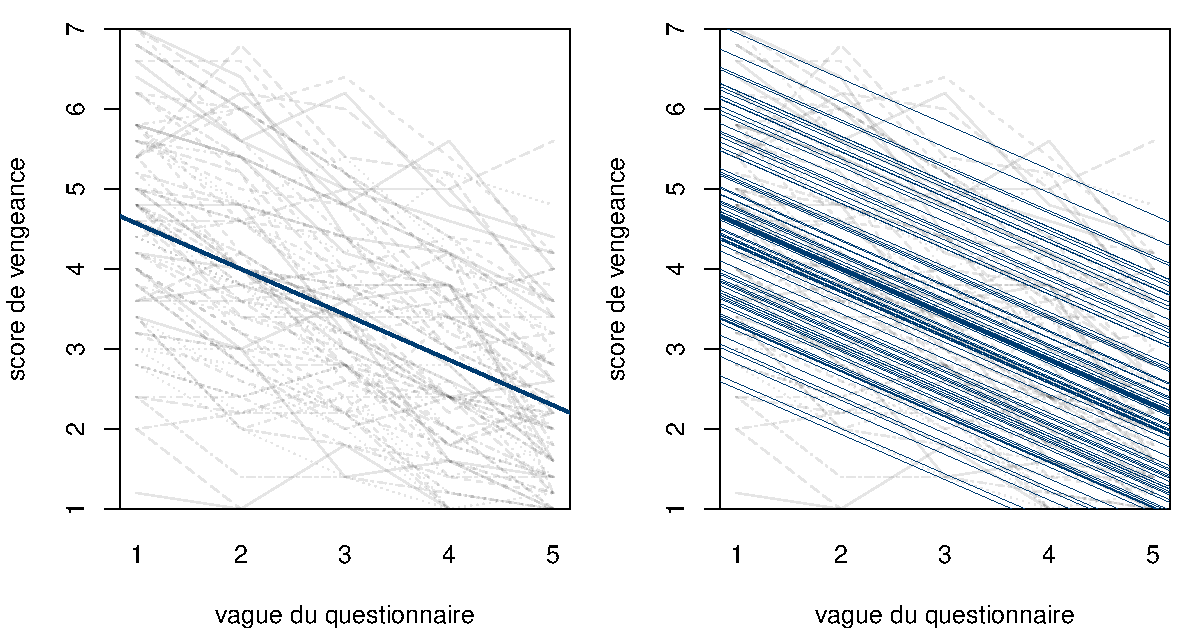
\includegraphics[width = 0.8\linewidth]{img/c6/07-mixed-randomintercept_fr}
\end{center}
{
\footnotesize Modèle sans effet aléatoire (gauche) et avec effet aléatoire pour \texttt{id} (droite).

}
\end{frame}
\begin{frame}[fragile]
\frametitle{Modèle avec ordonnée à l'origine aléatoire}
Soit l'équation du modèle,
\begin{align*}
Y_{ij}=(\beta_0+b_i)+ \beta_1 \mathrm{X}_{ij1}+\beta_2\mathrm{X}_{ij2}+\cdots+\beta_p\mathrm{X}_{ijp} + \varepsilon_{ij}
\end{align*}
\bi
\item Les effets aléatoires $b_1, \ldots, b_m$ sont supposées indépendants des termes d'aléas $\varepsilon$ et des variables explicatives
\item On postule  pour le moment 
\bi \item $b_{i\phantom{j}}\simiid \mathsf{No}(0, \sigma^2_b)$ $(i=1, \ldots, m)$.
\item $\varepsilon_{ij}\simiid \mathsf{No}(0, \sigma^2)$ $(i=1, \ldots, m; j = 1, \ldots, n_i)$.
\ei
% \item Les aléas $\varepsilon_{ij}$ pourraient être corrélées au sein du groupe $i$, mais on postule qu'ils sont indépendants pour le moment.
\ei
\end{frame}


\begin{frame}[fragile]
\frametitle{Modèles avec effets aléatoires: covariance}
Comme il est aléatoire, le terme $b_i$ introduit de la \alert{corrélation intra-groupe}
dans le modèle.  Puisque $\eps_{ij}$ est indépendant de $b_i$ pour tout $i, j$, la variance (conditionelle) d'une observation est
\begin{align*}
\Va{Y_{ij}\mid \mathbf{X}_i}&=\Va{b_i}+\Va{\varepsilon_{ij}}=\sigma^2_b + \sigma^2_{\vphantom{b}}
\end{align*}
La covariance entre deux individus d'un même groupe est
\begin{align*}
\Co{Y_{ij}, Y_{ik}\mid \mathbf{X}_i}=\sigma^2_b, \qquad j\neq k.
\end{align*}
Par conséquent, la corrélation entre deux individus d'un même groupe est
\begin{align*}
\Cor{Y_{ij}, Y_{ik}\mid \mathbf{X}_i}=\frac{\sigma^2_b}{\sigma^2_{\vphantom{b}}+\sigma^2_b}, \qquad  j\neq k.
\end{align*}
Cette quantité est habituellement appelée \alert{corrélation intra-groupe}.

\end{frame}

\begin{frame}{Aparté mathématique}
Les coefficients $\beta_j$ et les covariables ne sont pas aléatoires, ce qui fait que
 \begin{align*}
  \Co{Y_{ij}, Y_{ik} \mid \mathbf{X}_i} &= \mathsf{Co}\left(\beta_0 +b_i + \beta_1\mathrm{X}_{ij1}+\cdots + \eps_{ij},\right.\\
  & \quad \qquad \left.\beta_0 +b_i + \beta_1\mathrm{X}_{ik1}+\cdots + \eps_{ik} \mid \mathbf{X}_i\right)
  \\&= \Co{b_i+ \eps_{ij}, b_i + \eps_{ik}}
  \\&= \Va{b_i} + \Co{\eps_{ij}, \eps_{ik}} \\&= \sigma^2_b +\sigma^2\I{j=k}.
\end{align*}
où la dernière étape vient de l'indépendance entre $b_i$ et $\bs{\eps}$ et puisque $\Co{Y_{ij},Y_{ij}}=\Va{Y_{ij}}$.

\end{frame}
\begin{frame}{Variabilité des $\bs{Y}$}


De manière équivalente, on peut écrire
\begin{align*}
   \Va{\bs{Y}_i \mid \mathbf{X}_i} &= \Va{b_i \bs{1}_{n_i}} + \Va{\bs{\eps}_i}
%    \\&=
%    \begin{matrix} b_i \\ \vdots \\ b_i 
%    \end{matrix}
%    } + \Va{\begin{matrix}\eps_{i1} \\ \vdots \\ \eps_{in_i}\end{matrix}}
   \\&= \sigma^2_b \bs{1}_{n_i}\bs{1}_{n_i}^\top + \sigma^2 \mathbf{I}_{n_i}
   \\&= 
   \begin{pmatrix}
 \sigma^2_b &  \sigma^2_b & \cdots & \sigma^2_b \\
  \sigma^2_b &  \sigma^2_b & \cdots & \sigma^2_b \\
 \vdots & \ddots & \ddots & \vdots \\
 \sigma^2_b &  \sigma^2_b & \cdots & \sigma^2_b   
 \end{pmatrix} + \begin{pmatrix}
 \sigma^2 & 0 & \cdots &0\\
 0 & \sigma^2 & \ddots &0\\
 \vdots &\ddots & \ddots & \vdots\\
 0 & 0 & \cdots & \sigma^2
 \end{pmatrix}.
\end{align*}

\end{frame}

\begin{frame}[fragile]
\frametitle{Structure d'équicorrélation avec ordonnée à l'origine aléatoire}
\bi \item Quand les aléas $\bs{\eps}_i$ sont indépendants et homoscédastiques, soit $\Va{\bs{\eps}_i}=\sigma^2\mathbf{I}_{n_i}$, introduire un effet aléatoire pour l'ordonnée à l'origine fait en sorte que la corrélation intra-groupe est constante.
\item 
Dans ce cas précis, la matrice de covariance conditionnelle de  $\boldsymbol{Y}_i$ est donc la même que si
on considérait une régression linéaire sans effet aléatoire avec une structure d'équicorrélation pour  $\Va{\bs{\eps}_i}$.
\item 
La différence ici est que la corrélation doit être non-négative. Ce n'est généralement pas une limitation, car les corrélations intra-groupe ont tendance à être positives.
\ei
\end{frame}
% \begin{frame}[fragile]
% \frametitle{Structure d'équicorrélation du modèle avec ordonnée à l'origine aléatoire}
% \bi
% \item Nous voyons donc que l'introduction d'un effet aléatoire pour l'ordonnée à l'origine
% fait en sorte que les observations des individus d'un même groupe sont
% corrélées et que \alert{la corrélation est la même} peu importe les individus choisis (équicorrélation).
% \item Ainsi, \textbf{ajouter un effet aléatoire pour l'ordonnée à l'origine revient à utiliser une
% structure d'équicorrélation}.
% \ei 
% \end{frame}
% \begin{frame}
% \frametitle{Équicorrélation}
% \bi 
% \item La différence ici est que la corrélation doit nécessairement être
% plus grande ou égale à zéro sachant que le $\sigma^2_b$ est une variance et donc forcément positive, alors que dans le  modèle d'équicorrélation, on a
% \[-\frac{1}{\max\{n_1, \ldots, n_m\}-1} \leq \rho \leq 1.\]
% \item Ce n'est généralement pas une limitation, car les corrélations intra-groupe ont tendance à être positives.
% 
% \ei
% \end{frame}


\begin{frame}[fragile]
\frametitle{Ajout d'un effet aléatoire avec la commande \code{random}}
\bi
\item La commande \code{repeated} nous permettait de spécifier la structure de covariance des erreurs avec \code{proc mixed}.
\item Si on utilise pas la commande \texttt{repeated}, les erreurs sont postulées indépendantes.
\ei
\begin{tcolorbox}[colback=white, colframe=hecblue, title=Code \SASlang pour ajuster un modèle avec ordonnée à l'origine aléatoire avec erreurs indépendantes]
\begin{footnotesize}
\begin{verbatim}
proc mixed data=modstat.mobilisation;
class idunite;
model mobilisation = sexe anciennete agegest nunite / solution;
random intercept / subject=idunite v=1 vcorr=1;
run;
\end{verbatim}
\end{footnotesize}
\end{tcolorbox}
{\footnotesize L'inclusion d'une ordonnée à l'origine aléatoire \alert{induit} une structure d'équicorrélation pour les réponses. Il n'est donc pas nécessaire de spécifier une structure de covariance pour les erreurs.

}
\end{frame}

\begin{frame}[fragile]
\frametitle{Matrice de covariance du modèle avec ordonnée à l'origine aléatoire}
\begin{center}
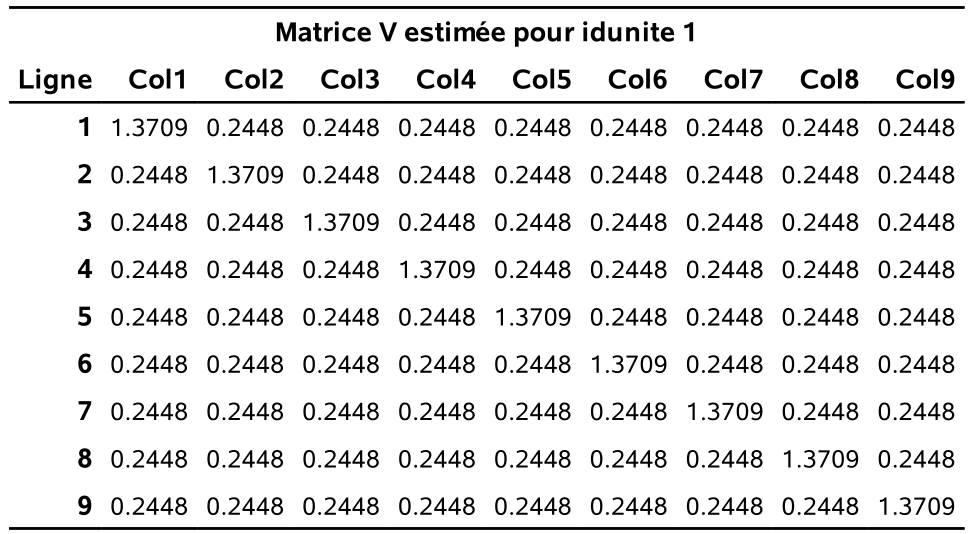
\includegraphics[width = 0.9\linewidth]{img/c6/diapos7-e11}

\end{center}
\end{frame}


\begin{frame}[fragile]
\frametitle{Estimés des paramètres de covariance}
\begin{center}
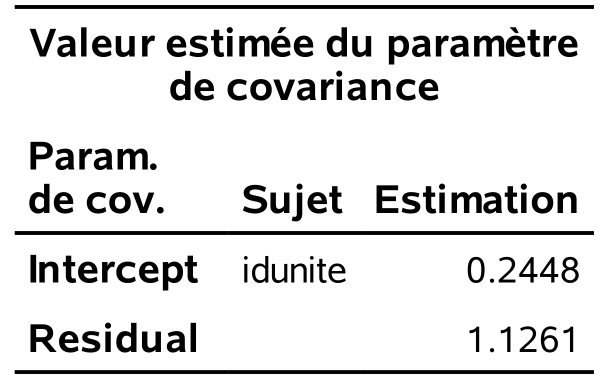
\includegraphics[width = 0.4\linewidth]{img/c6/diapos7-e12}
\end{center}
\bi
\item L'estimé de la variance de l'effet aléatoire est
$\hat{\sigma}^2_b=0,2448$, tandis que l'estimé de la variance des erreurs est
$\hat{\sigma}^2= 1,1261$.
\item Conséquemment, la corrélation intra-unité est
\begin{align*}
\hat{\rho}=\frac{\hat{\sigma}^2_b}{\hat{\sigma}^2_b+\sigma^2_{\vphantom{b}}}=0,1785.
\end{align*}

\item C'est exactement la même corrélation que celle rapportée pour le modèle d'équicorrélation intra-unité des erreurs (commande \code{repeated}).
\ei
\end{frame}

\begin{frame}[fragile]
\frametitle{Estimés des effets fixes}
\begin{center}
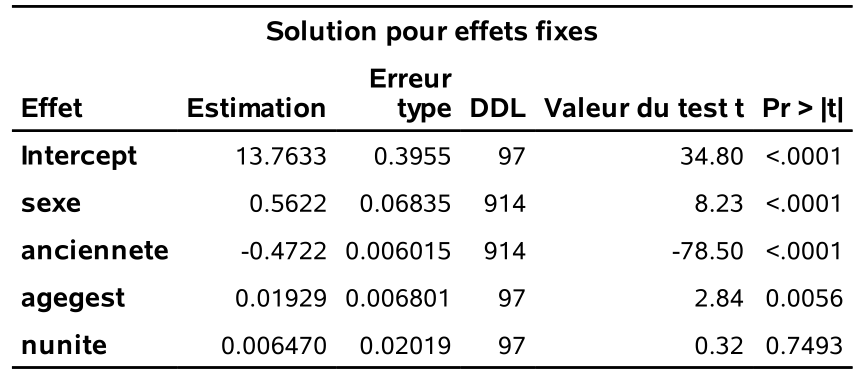
\includegraphics[width = 0.7\linewidth]{img/c6/diapos7-e10}
\end{center}
{\footnotesize L'effet des variables explicatives (et leurs erreurs-types) sont exactement les même que pour le modèle d'équicorrélation des erreurs --- les deux modèles sont équivalents pour la réponse si la corrélation intra-unité est positive.


}
\end{frame}
%  \begin{frame}
% \frametitle{Modèle pour données longitudinales \texttt{vengeance}}
% \bi
% \item Dans le cas de données longitudinale, spécifier une structure $\mathsf{AR}(1)$ pour les données peut se faire en ajoutant une structure sur les résidus du modèle, \alert{en plus de la spécification des effets aléatoires}.
% \item Le structure du modèle est
% \begin{align*}
% Y_{ij}=\beta_0 +b_i + \beta_1 \mathrm{X}_{ij1}+\beta_2\mathrm{X}_{ij2}+\cdots+\beta_p\mathrm{X}_{ijp} + \varepsilon_{ij}
% \end{align*}
% mais on suppose que
% \bi
% 
% \item l'ordonnée à l'origine aléatoire $b_{i} \simiid \mathsf{No}(0, \sigma^2_b)$,
% \item  les erreurs $\bs{\varepsilon}_i \sim \mathsf{No}\big(\bs{0}_{n_i}, \bs{\Sigma}_i\big)$,
% \item $\varepsilon_{ij}$ sont \alert{dépendants} au sein de l'individu $i$ --- $\bs{\Sigma}_i$ n'est pas diagonale.
% \ei
% \item On postule une strucutre $\mathsf{AR}(1)$ (mais cela pourrait être un autre modèle, pourvu qu'il soit différent du modèle d'équicorrélation) pour la matrice de covariance intra-individu des erreurs, $\bs{\Sigma}_i$.
% \ei
% 
% {\footnotesize Remarque:
%   bien que les paramètres des matrices de covariance intra-groupe $\bs{\Sigma}_i$ soit potentiellement partagées, ces matrices peuvent être de taille différentes.
% 
%  }
% \end{frame}
% 
% \begin{frame}[fragile]
% \frametitle{Ordonnée à l'origine aléatoire avec structure $\mathsf{AR}(1)$ pour les erreurs}
% \begin{tcolorbox}[colback=white, colframe=hecblue, title=Code \SASlang pour l'ordonnée à l'origine aléatoire avec erreurs $\mathsf{AR}(1)$]
% \begin{verbatim}
% proc mixed data=vengeance;
% class id tcat;
% model vengeance = sexe age vc wom t / solution;
% random intercept / subject=id v=1 vcorr=1;
% repeated tcat / subject=id type=ar(1) r=1 rcorr=1;
% run;
% \end{verbatim}
% \end{tcolorbox}
% 
% \bi
% \item L'option \texttt{v=1 vcorr=1} demande à \SASlang{} d'afficher la matrice de covariance/corrélation des \alert{observations $Y$} pour le sujet $1$.
% \item L'option \texttt{r=1 rcorr=1} demande à \SASlang{} d'afficher la matrice de covariance/corrélation des \alert{erreurs $\bs{\epsilon}$} pour le sujet $1$.
% \ei
% \end{frame}
% 
% \begin{frame}[fragile]
% \frametitle{Matrices de covariance et de corrélation des \textbf{erreurs}}
% \begin{center}
% 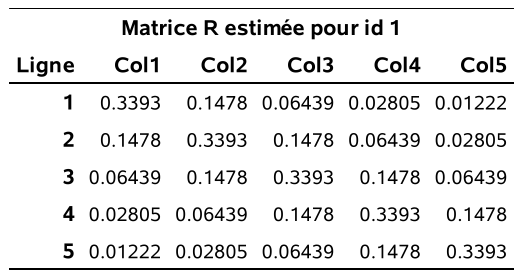
\includegraphics[width=0.49\linewidth]{img/c6/diapos7-e13}
% 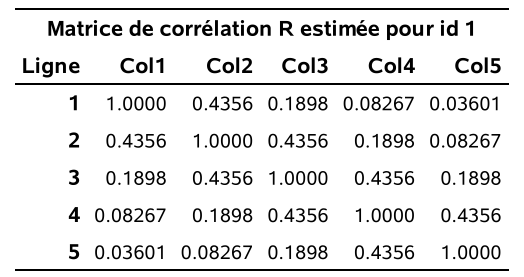
\includegraphics[width=0.49\linewidth]{img/c6/diapos7-e14}
% \end{center}
% 
% \end{frame}
% 
% \begin{frame}[fragile]
% \frametitle{Matrices de covariance et de corrélation des \textbf{observations}}
% \begin{center}
% 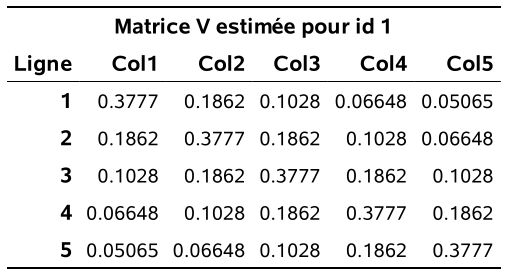
\includegraphics[width=0.50\linewidth]{img/c6/diapos7-e15}
% 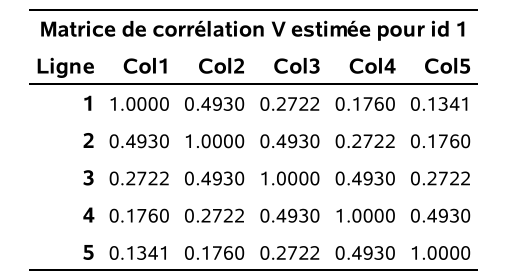
\includegraphics[width=0.49\linewidth]{img/c6/diapos7-e16}
% \end{center}
% \bi
% \item Ces matrices sont différentes de celles des erreurs (diapositive précédente).
% \item La covariance des \alert{observations} est la somme de la covariance des effets aléatoires et de la covariance des résidus.
% \ei
% \end{frame}
% 
% 
% % \begin{frame}[fragile]
% % \frametitle{Covariance parameters}
% % \begin{center}
% % \includegraphics[scale=0.8]{img/c6/long123_5.pdf}
% % \end{center}
% % There are three covariance parameters in the model:
% % \bi
% % \item The variance of the random effect $\hat{\sigma}^2_b=0.038$ (not significant).
% % \bi \item[] \textbf{warning: non-regular test, unreliable output!}\ei
% % \item The variance of the residuals $\varepsilon$, $\hat{\sigma}^2_e$, is $0.33$.
% % \item The lag-one correlation $\hat{\rho}=0.43$ of the $\mathsf{AR}(1)$ model (significant).
% % \ei
% % \end{frame}
% \begin{frame}[fragile]
% \frametitle{Paramètres de covariance}
% \begin{center}
% 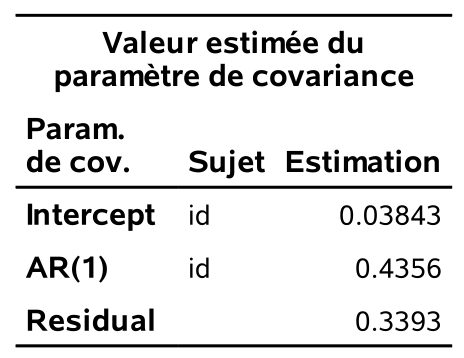
\includegraphics[width = 0.4\linewidth]{img/c6/diapos7-e17}
% \end{center}
% Il y a trois paramètres de covariance dans le modèle, dont les estimés sont
% \bi
% \item pour la variance de l'effet aléatoire pour l'ordonnée à l'origine, $\hat{\sigma}^2_b=0,038$.
% \item pour la variance des erreurs $\varepsilon$, $\hat{\sigma}^2=0,33$.
% \item pour la corrélation à un pas de temps du modèle $\mathsf{AR}(1)$, $\hat{\rho}=0,43$.
% \ei
% \end{frame}
% \begin{frame}[fragile]
% \frametitle{Critères d'information et estimés des effets fixes}
% \begin{center}
% 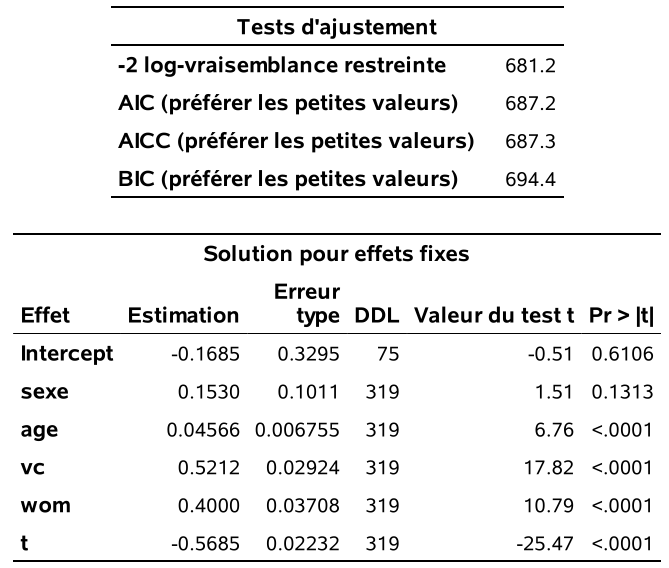
\includegraphics[width =0.6\linewidth]{img/c6/diapos7-e18}
% \end{center}
% {\footnotesize
% Les estimés sont pour le modèle mixte avec ordonnée à l'origine aléatoire (pour \texttt{id}) et un modèle de covariance $\mathsf{AR}(1)$ pour les erreurs. On pourrait comparer ce modèle à celui du Chapitre 6 qui n'incluait pas d'effet aléatoire.
% 
% }
% \end{frame}
% 
% 
% % \begin{frame}[fragile]
% % \frametitle{Investigation of the usefulness of the random intercept}
% % \bi
% % \item Testing whether the variance of the random effect $\sigma^2_b=0$ (corresponding to no random intercept) is a non-standard testing problem \ldots
% % \item The model which includes a random intercept et an $\mathsf{AR}(1)$ covariance structure within-unit for the residuals had a $\mathsf{BIC}$ ($\mathsf{AIC}$) of $694.4$ ($687.2$) compared to $690.5$ ($685.8$) for the model that assumes independent residuals.
% % \item According to the $\mathsf{BIC}$, the best model is the one without a random effect, but with an $\mathsf{AR}(1)$ correlation on the errors. $\mathsf{AIC}$ prefers more complicated models et so includes the random intercept.
% % \item It seems that modelling an intercept for each subject is not necessary in this example. The $\mathsf{AR}(1)$ correlation of the errors appears to be sufficient in explaining the correlation in the data.
% % \ei
% % \end{frame}
% \begin{frame}
%  \frametitle{Effet fixe ou aléatoire?}
%  \bi \item La théorie se généralise à des cas plus complexes (pentes aléatoires par groupe).
%  \item Si on doit choisir entre ajouter un effet fixe (ou aléatoire) pour une variable (effet groupe), il faut garder en tête les règles de base suivantes:
%  \bi
% 
%  \item les \textbf{effets fixes} de groupe sont utilisés dans les cas où on a peu de groupes et beaucoup d'observations dans chacun. On s'intéresse aussi à l'effet groupe en tant que tel (petit $m$, grande taille d'échantillon  $n_i$ pour chaque groupe).
%  \item les \textbf{effets aléatoires} sont utilisés quand on a suffisamment de niveaux pour le facteur groupe afin d'estimer de façon fiable la variance $\sigma^2_b$; l'effet groupe n'est pas intéressant en tant que tel ($m$ grand, taille d'échantillon du groupe $n_i$ petite).
%  \ei
%  \item Tester si l'effet aléatoire est nécessaire ou pas revient à tester si sa variance est nulle, soit $\sigma^2_b=0$; c'est un test d'hypothèse non-standard, qui est au delà du niveau du cours\ldots
%  \ei
% \end{frame}
% 
% 
% \begin{frame}
% \frametitle{Moyenne marginale et conditionnelle}
% \bi
% \item Au niveau de la population, la \alert{moyenne marginale} de $Y_{ij}$ est, comme à l'accoutumée,
% \begin{align*}
% \E{Y_{ij}\mid \mathbf{X}_i}=\beta_0  + \beta_1 \mathrm{X}_{ij1}+\beta_2\mathrm{X}_{ij2}+\cdots+\beta_p\mathrm{X}_{ijp}.
% \end{align*}
% \item En revanche, la \alert{moyenne conditionelle} de $Y_{ij}$, sachant l'effet spécificque à son groupe, est
% \begin{align*}
% \E{Y_{ij}\mid \mathbf{X}_i, b_{i}}&=(\beta_0 + \alert{b_i}) + \beta_1 \mathrm{X}_{ij1}+\cdots+\beta_p\mathrm{X}_{ijp}.
% \end{align*}
% \item En \textbf{prédisant} $b_{i}$, on peut prédire la valeur de $Y_{ij}$ tout en prenant en compte l'effet aléatoire spécifique au groupe pour l'ordonnée à l'origine.
% \ei
% \end{frame}


\end{document}
